%!TEX root = report.tex

\chapter{Spécification des besoins}


Dans ce chapitre on présente les environnements logiciels et matériels dans lesquelles s'est dérouler le développement de l'application ainsi qu'une étude des besoins effectué pour cerner nos objectifs.

\section{Environnement de développement}%TODO

Plusieurs outils ont été mises à contribution pour développer l'application, tant sur le plan logiciel que matériel.

\subsection{Environnement Logiciel}
Voici une liste des outils logiciels utilisés pendant le développement de l'application.

\begin{description}

\item [Ubuntu 12.04] Système d'exploitation.\footnotemark[1]

\item [OpenJDK 6] \gls{jdk} version 6.\footnotemark[2]

\item [Eclipse Juno] Environnement de Développement Intégré dans sa version \en{Service Release 2}.\footnotemark[3]

\item [\gls{adt} (plugin Eclipce)] Intégration des outils de développement fournit dans l'\gls{sdk} \android{}.\footnotemark[4]

\item [ObjectAid (plugin Eclipce)] Génération des diagrammes de classes.\footnotemark[5]

\item [PlantUML (plugin Eclipce)] Génération des diagrammes de séquences.\footnotemark[6]

\item [Git] Gestionnaire des versions\footnotemark[7].

\item [EGit (plugin Eclipse)] Intégration du gestionnaire de version.\footnotemark[8]

\item [Evolus Pencil] Génération de prototypes et des sketchs\footnotemark[9]
\end{description}

\footnotetext[1]{http://www.ubuntu.com}
\footnotetext[2]{http://openjdk.java.net}
\footnotetext[3]{http://www.eclipse.org}
\footnotetext[4]{https://developer.android.com/tools/sdk/eclipse-adt.html}
\footnotetext[5]{http://www.objectaid.com/}
\footnotetext[6]{http://plantuml.sourceforge.net/}
\footnotetext[7]{ttp://git-csm.com}
\footnotetext[8]{http://www.eclipse.org/egit/}
\footnotetext[9]{http://pencil.evolus.vn/}

\subsection{Environnement Matériel}

Le développement de l'application est fait avec une tablette Asus Nexus 7 (mise à jour à \android{} 4.2.2 \en{Jelly Bean}).


\section{Étude des Besoins}

\subsection{Besoins fonctionnels}

\begin{figure}[H]
\center
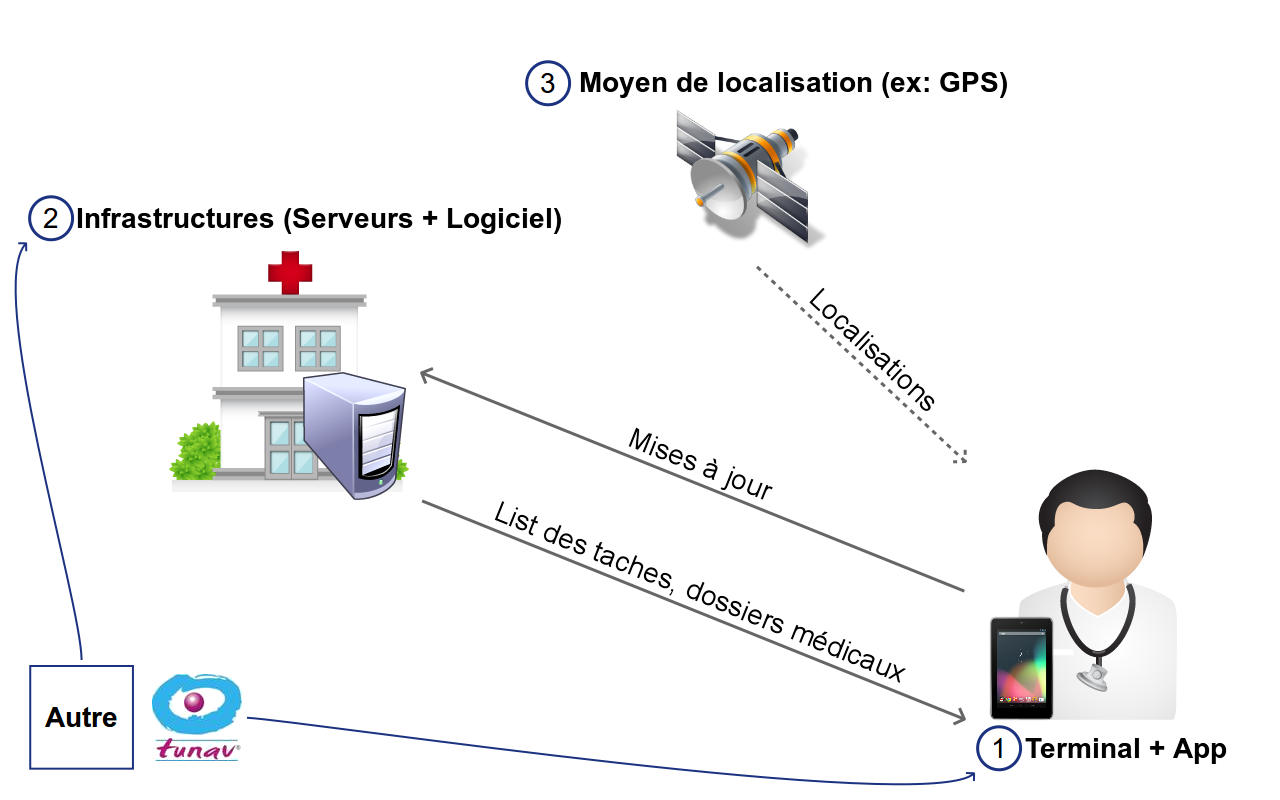
\includegraphics[width=0.8\textwidth]{scenario-other}
\caption{Illustration des besoins fonctionnels.}
\end{figure}

\begin{itemize}

\item Le médecin doit être capable à partir de son terminal d’avoir des
informations sur les patients qui lui sont assignés en fonction de leur position
géographique.

\item L'application doit être capable de détecter la proximité d'un
patient en fonction de la position actuelle du terminal.

\item Le médecin peut télé-consulter le dossier médical du patient.

\end{itemize}

\subsection{Besoins non fonctionnels}

\begin{itemize}

\item Une bonne ergonomie qui vise à faciliter l'obtention de
l'information, avec un minimum d'effort pour l'utilisateur cible et
avec le moindre risque d'erreur. Les choix graphiques et conceptuels
sont des considérations à tenir en compte.

\end{itemize}

\subsection{Besoins techniques}

\begin{figure}[H]
\center
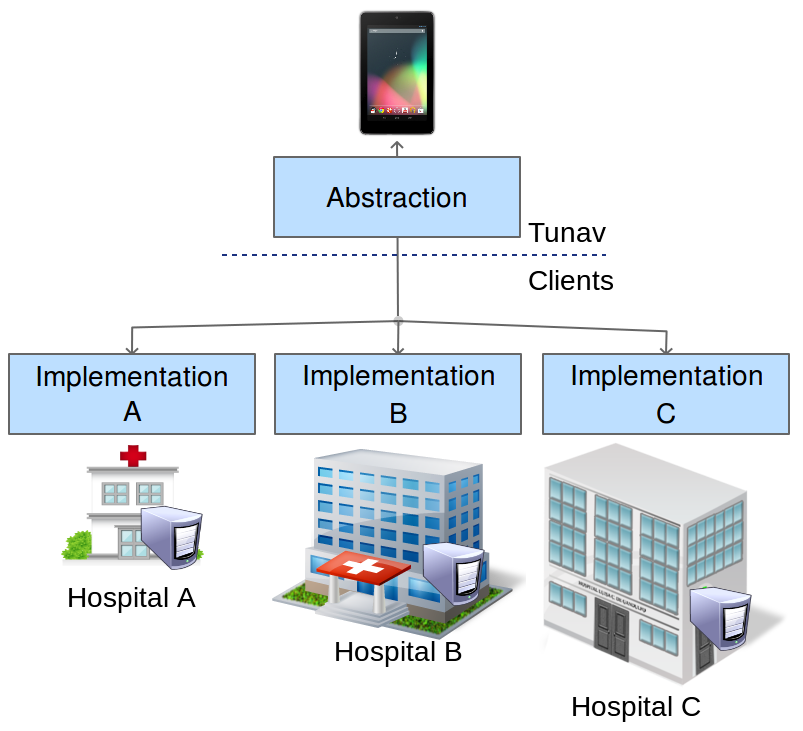
\includegraphics[width=0.8\textwidth]{architecture-interfaces}
\caption{Illustration des besoins techniques.}
\end{figure}

\begin{itemize}

\item L’application mobile vise à utiliser les systèmes déjà en place des
établissements clients pour réduire les coûts. Vu l’absence d'un protocole
standards et les différentes implémentations possibles des différents clients,
l'implémentation d'une couche d’accès abstraite est requise pour pouvoir
déployer l’application avec le minimum de modification.

\end{itemize}

\subsection{Identification des acteurs}

Notre système interagit essentiellement avec trois acteurs différents:

\begin{description}

\item[Le médecin] C'est l'acteur principal de notre système.

\item[Le service web] Source des données à acheminer vers le médecin.

\item[Système d'exploitation] Communique à notre système les
informations recueillies des divers composants qui nous intéressent
(localisation GPS/Network, état de la connectivité, état de la
batterie).

\end{description}

\subsection{Cas d'utilisations}

On peut présenter les interactions fonctionnelles entre les acteurs gouverné par leurs besoins avec un diagramme des cas d'utilisations (figure \ref{fig:uml_usecase}).

\begin{figure}
\center
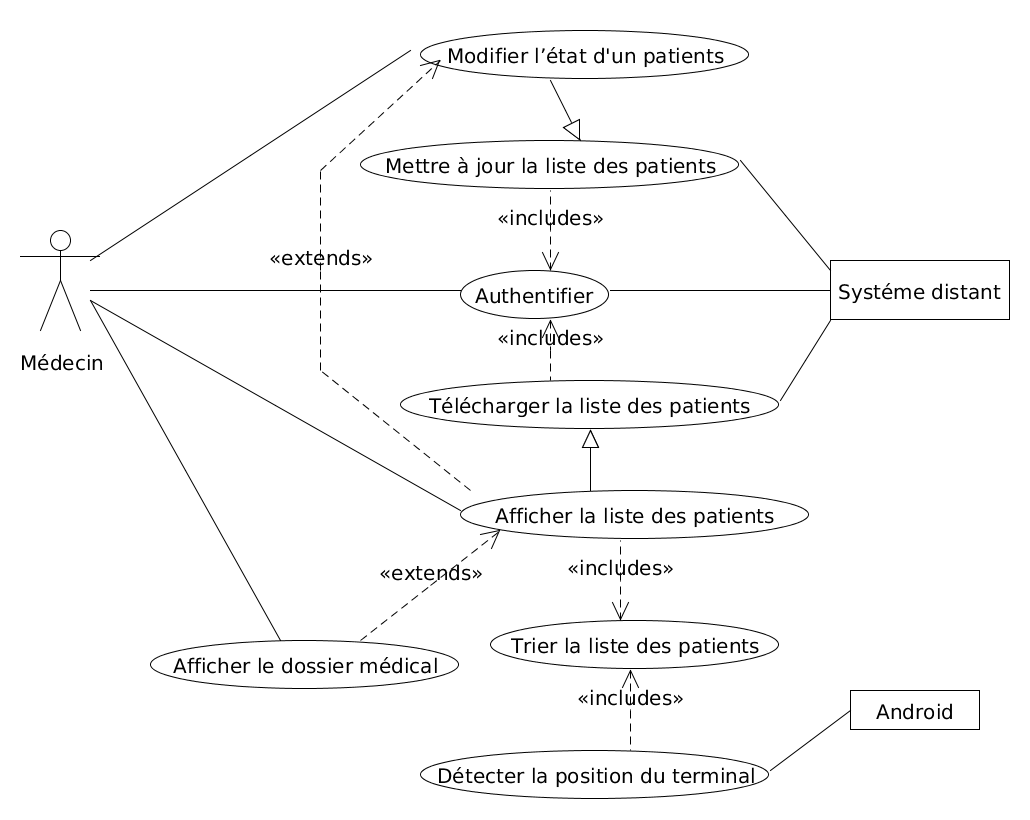
\includegraphics[width=0.8\textwidth]{diagrams/usecases}
\caption{Diagramme des cas d'utilisation \gls{uml} globale.}
\label{fig:uml_usecase}
\end{figure}